\begin{center}
\begin{tikzpicture}
	\node[anchor=south west,inner sep=0] (image)  at (0,0) {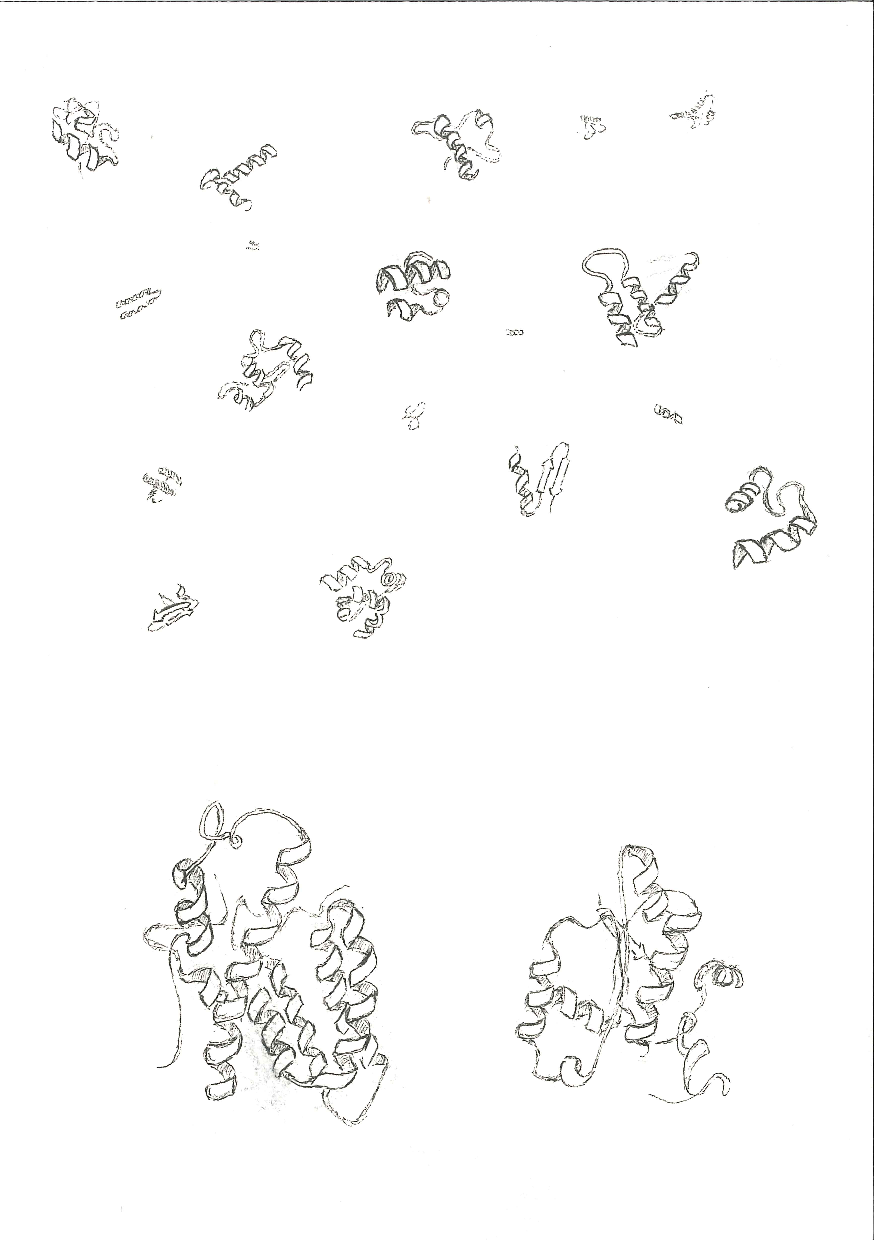
\includegraphics[trim={2mm, 2mm, 2mm, 2mm}, width=0.995\pagewidth]{scans/panel-7.pdf}};
    \begin{scope}[x={(current page.south east)},y={(current page.north west)}]
		\if\helplines1
			\draw[help lines,xstep=.1,ystep=.1] (0,0) grid (\N, \N);
		\else
			\path[help lines,xstep=.1,ystep=.1] (0,0) grid (\N, \N);
		\fi
		\node[text width=0.35\pagewidth, align=justify, anchor= west] at (0.07, 0.80) {\english{Once our pipeline was finished and validated, we launched it on all the \oldstylenums{6\,000} known protein families for which we don't know the structure.}};
		
		\node[text width=0.35\pagewidth, align=justify, anchor= east] at (1-0.07, 0.68) {\spanish{\oldstylenums{Una vez que validamos el protocolo, lo usamos para intentar predecir todas las 6\,000 familias de proteínas de las que no conozemos la estructura.}}};
		
		\node[text width=0.4\pagewidth, align=justify, anchor= west] at (0.075, 0.4) {\english{We believe over 500 of those are accurate models, of which 415 were never reported before.}};
		
		\node[text width=0.4\pagewidth, align=justify, anchor= east] at (1-0.075, 0.4) {\spanish{\oldstylenums{Creemos que para 500 de ellas, nuestros modelos son precisos. De estas, 415 nunca habían sido presentadas antes.}}};
		
    \end{scope}

\end{tikzpicture}
\end{center}
